% latex_beamer_template_nociones_basicas.tex
% 2014-02-10 dmontaner@cipf.es
% Latex template to be used in combination with pandoc

% see for templates:
% http://deic.uab.es/~iblanes/beamer_gallery/
% see for colors:
% http://deic.uab.es/~iblanes/beamer_gallery/index_by_color.html

%% Parece que los temas se almacenan en este dir:
%% /usr/share/texmf/tex/latex/beamer/base/themes

%% tree /usr/share/texmf/tex/latex/beamer/base/themes
%% ├── color
%% │   ├── beamercolortheme...albatross.sty
%% │   ├── beamercolortheme...beaver.sty
%% │   ├── beamercolortheme...beetle.sty
%% │   ├── beamercolortheme...crane.sty
%% │   ├── beamercolortheme...default.sty
%% │   ├── beamercolortheme...dolphin.sty
%% │   ├── beamercolortheme...dove.sty
%% │   ├── beamercolortheme...fly.sty
%% │   ├── beamercolortheme...lily.sty
%% │   ├── beamercolortheme...monarca.sty
%% │   ├── beamercolortheme...orchid.sty
%% │   ├── beamercolortheme...rose.sty
%% │   ├── beamercolortheme...seagull.sty
%% │   ├── beamercolortheme...seahorse.sty
%% │   ├── beamercolortheme...sidebartab.sty
%% │   ├── beamercolortheme...spruce.sty
%% │   ├── beamercolortheme...structure.sty
%% │   ├── beamercolortheme...whale.sty
%% │   └── beamercolortheme...wolverine.sty
%% ├── font
%% │   ├── beamerfonttheme...default.sty
%% │   ├── beamerfonttheme...professionalfonts.sty
%% │   ├── beamerfonttheme...serif.sty
%% │   ├── beamerfonttheme...structurebold.sty
%% │   ├── beamerfonttheme...structureitalicserif.sty
%% │   └── beamerfonttheme...structuresmallcapsserif.sty
%% ├── inner
%% │   ├── beamerinnertheme...circles.sty
%% │   ├── beamerinnertheme...default.sty
%% │   ├── beamerinnertheme...inmargin.sty
%% │   ├── beamerinnertheme...rectangles.sty
%% │   └── beamerinnertheme...rounded.sty
%% ├── outer
%% │   ├── beameroutertheme...default.sty
%% │   ├── beameroutertheme...infolines.sty
%% │   ├── beameroutertheme...miniframes.sty
%% │   ├── beameroutertheme...shadow.sty
%% │   ├── beameroutertheme...sidebar.sty
%% │   ├── beameroutertheme...smoothbars.sty
%% │   ├── beameroutertheme...smoothtree.sty
%% │   ├── beameroutertheme...split.sty
%% │   └── beameroutertheme...tree.sty
%% └── theme
%%     ├── beamertheme...AnnArbor.sty
%%     ├── beamertheme...Antibes.sty
%%     ├── beamertheme...Bergen.sty
%%     ├── beamertheme...Berkeley.sty
%%     ├── beamertheme...Berlin.sty
%%     ├── beamertheme...Boadilla.sty
%%     ├── beamertheme...boxes.sty
%%     ├── beamertheme...CambridgeUS.sty
%%     ├── beamertheme...Copenhagen.sty
%%     ├── beamertheme...Darmstadt.sty
%%     ├── beamertheme...default.sty
%%     ├── beamertheme...Dresden.sty
%%     ├── beamertheme...EastLansing.sty
%%     ├── beamertheme...Frankfurt.sty
%%     ├── beamertheme...Goettingen.sty
%%     ├── beamertheme...Hannover.sty
%%     ├── beamertheme...Ilmenau.sty
%%     ├── beamertheme...JuanLesPins.sty
%%     ├── beamertheme...Luebeck.sty
%%     ├── beamertheme...Madrid.sty
%%     ├── beamertheme...Malmoe.sty
%%     ├── beamertheme...Marburg.sty
%%     ├── beamertheme...Montpellier.sty
%%     ├── beamertheme...PaloAlto.sty
%%     ├── beamertheme...Pittsburgh.sty
%%     ├── beamertheme...Rochester.sty
%%     ├── beamertheme...Singapore.sty
%%     ├── beamertheme...Szeged.sty
%%     ├── beamertheme...Warsaw.sty
%%     └── compatibility
%%         ├── beamertheme...bars.sty
%%         ├── beamertheme...classic.sty
%%         ├── beamertheme...compatibility.sty
%%         ├── beamertheme...lined.sty
%%         ├── beamertheme...plain.sty
%%         ├── beamertheme...shadow.sty
%%         ├── beamertheme...sidebar.sty
%%         ├── beamertheme...split.sty
%%         └── beamertheme...tree.sty


%% Inner Themes
%% ================================================================================

%% An inner theme installs templates that dictate how the following elements are typeset:
%% - Title and part pages.
%% - Itemize environments.
%% - Enumerate environments.
%% - Description environments.
%% - Block environments.
%% - Theorem and proof environments.
%% - Figures and tables.
%% - Footnotes.
%% - Bibliography entries.


%% Outer Themes
%% ================================================================================
%% An outer theme dictates the overall layout of frames. 
%% It specifies where any navigational elements should go 
%% and what they should look like. 

%% An outer theme specifies how the following elements are rendered:
%% - The head- and footline.
%% - The sidebars.
%% - The logo.
%% - The frame title.


%%%%%%%%%%%%%%%%%%%%%%%%%%%%%%%%%%%%%%%%%%%%%%%%%%%%%%%%%%%%%%%%%%%%%%%%%%%%%%%%
%%% TEMPLATE
%%%%%%%%%%%%%%%%%%%%%%%%%%%%%%%%%%%%%%%%%%%%%%%%%%%%%%%%%%%%%%%%%%%%%%%%%%%%%%%%

\documentclass{beamer}
\usepackage[utf8]{inputenc}
\usepackage[T1]{fontenc}
\usepackage{lmodern}  %use allways with T1. Otherwhise the letter looks whiard.

%\usepackage[spanish]{babel} %NOT WORKING

%% \usepackage{longtable}

%% \makeatletter 
%% \def\fnum@table{\tablename~\thetable} 
%% \makeatother 



%% INNER theme
%\useinnertheme{rounded}         %bullets as balls, round borders
\useinnertheme[shadow]{rounded}  %shadow under the boxes

%% OUTER theme
\useoutertheme{shadow} % shadow under the titles and some color gradient as well for them.

%% FONT theme
%\usefonttheme{default}      % sans serif font f
\usefonttheme{structurebold} % NICE

%% COLOR theme
%\usecolortheme{default}
%\usecolortheme{orchid}    % blanco como el default ???
%
%\usecolortheme{whale}     % blue dark NICE
%\usecolortheme{seahorse}  % blue light
%
\usecolortheme{crane}      % orange NICE
%\usecolortheme{wolverine} % yellow
%
%\usecolortheme{fly}       % grey NICE
%\usecolortheme{beetle}    % grey NICE blue headers

%% more BEAMER theme:
%% (set after the theme selection)
\setbeamertemplate{frametitle}[default][center]    % center titles

\definecolor{links}{HTML}{2A1B81}                  % hyperref colors
\hypersetup{colorlinks,linkcolor=,urlcolor=links}

\setbeamertemplate{navigation symbols}{}           %%suppresses all navigation symbols

%%%%%%%%%%%%%%%%%%%%%%%%%%%%%%%%%%%%%%%%%%%%%%%%%%%%%%%%%%%%%%%%%%%%%%%%%%%%%%%%

%% TITLE etc
%% \title[título corto]{Titulo Largo de la Presentación}
%% \title[NCBI databases \hspace{2em} \insertframenumber\ / \inserttotalframenumber]{Titulo Largo de la Presentación}
%% \subtitle{subtitulo}
%% \author[Estudios Insilico en Biomedicina\hspace{8em}]{David Montaner}
%% \date{February 14, 2008}


%%%%%%%%%%%%%%%%%%%%%%%%%%%%%%%%%%%%%%%%%%%%%%%%%%%%%%%%%%%%%%%%%%%%%%%%%%%%%%%%
%%% DOCUMENT
%%%%%%%%%%%%%%%%%%%%%%%%%%%%%%%%%%%%%%%%%%%%%%%%%%%%%%%%%%%%%%%%%%%%%%%%%%%%%%%%
\begin{document}

\input{"010_title.tex"}

\title[\hspace{2em} NGS data anlysis course \hspace{8em} \insertframenumber\ / \inserttotalframenumber]{NGS data anlysis course}

\subtitle{{\color{gray}\titulolargo}} %% GREY is nice for the 'whale' and the 'crane' color themes

\author[\titulocorto \hspace{2em}]{
\href{http://www.dmontaner.com}{Ignacio Medina} \\
\href{http://www.dmontaner.com}{David Montaner}  
 \& \href{http://www.dmontaner.com}{Marta Bleda}}

%% \author[Transcriptomics \hspace{2em}]{\href{http://ngscourse.github.io/}{ngscourse.github.io}}

\date{
\includegraphics[width=0.2\textwidth]{../../../course_commons/logo_cipf.png}}

\begin{frame}
  \maketitle
\end{frame}

\begin{frame}[fragile]{Some syntax}

\href{http://johnmacfarlane.net/pandoc/demo/example9/pandocs-markdown.html}{See
Pandoc markdown syntax here}

~

\emph{italics}

\textbf{bold}

\begin{verbatim}
verbatim
\end{verbatim}

No break paragraph like this.

But with 2 spaces\\at the end of the line.

vertical

~

space

\end{frame}

\begin{frame}{Slide with bullets}

\begin{itemize}
\itemsep1pt\parskip0pt\parsep0pt
\item
  one
\item
  two
\item
  three

  \begin{itemize}
  \itemsep1pt\parskip0pt\parsep0pt
  \item
    and a second level
  \item
    and more \ldots{}
  \end{itemize}
\end{itemize}

\begin{enumerate}
\def\labelenumi{\arabic{enumi}.}
\itemsep1pt\parskip0pt\parsep0pt
\item
  ONE
\item
  TWO
\item
  THREE
\end{enumerate}

\end{frame}

\begin{frame}[fragile]{Slide with subsections}

\begin{block}{Subsection one}

\begin{itemize}
\itemsep1pt\parskip0pt\parsep0pt
\item
  something here
\item
  more here
\end{itemize}

\end{block}

\begin{block}{Subsection two}

\begin{verbatim}
verbatim here
more
\end{verbatim}

\end{block}

\end{frame}

\begin{frame}{Slide with hyperlinks}

\url{http://ngscourse.github.io}

\href{https://github.com}{Follow the link}

\href{https://github.com}{Follow the link}

\begin{block}{Reusable Link}

\href{https://github.com/ngscourse/ngscourse.github.io/blob/master/README.md}{readme}

\href{https://github.com/ngscourse/ngscourse.github.io/blob/master/README.md}{Readme}

\href{https://github.com/ngscourse/ngscourse.github.io/blob/master/README.md}{README}

\href{https://github.com/ngscourse/ngscourse.github.io/blob/master/README.md}{go
to the readme}

\end{block}

\end{frame}

\begin{frame}{Big Image}

\begin{figure}[htbp]
\centering

\includegraphics[width=\textwidth,height=0.8\textheight,keepaspectratio]{images/smile}
\caption{caption here: do not use it}
\end{figure}

\end{frame}

\begin{frame}{Small Image (PNG)}

\begin{figure}[htbp]
\centering

\includegraphics[width=\textwidth,height=0.8\textheight,keepaspectratio]{images/small}
\end{figure}

\end{frame}

\begin{frame}{Square Image}

\begin{figure}[htbp]
\centering

\includegraphics[width=\textwidth,height=0.8\textheight,keepaspectratio]{images/square}
\end{figure}

\end{frame}

\begin{frame}{Horizontal image}

\begin{figure}[htbp]
\centering

\includegraphics[width=\textwidth,height=0.8\textheight,keepaspectratio]{images/horizontal}
\end{figure}

\end{frame}

\begin{frame}{Vertical image}

\begin{figure}[htbp]
\centering
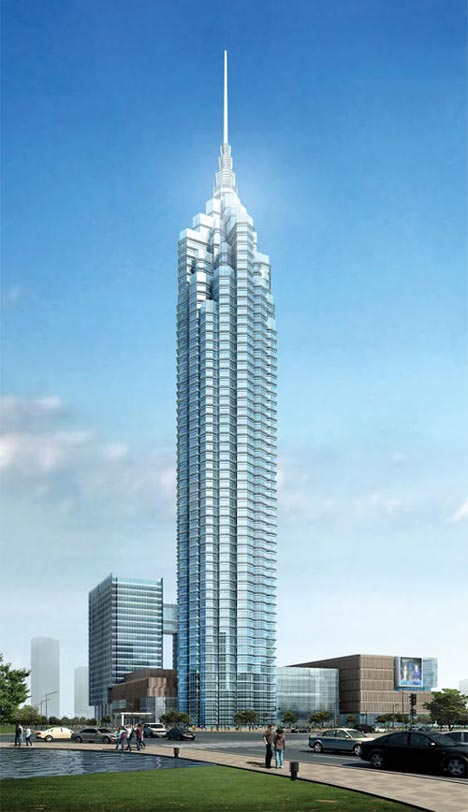
\includegraphics[width=\textwidth,height=0.8\textheight,keepaspectratio]{images/vertical}
\end{figure}

\end{frame}

\begin{frame}{SCALED image}

\centerline{
\includegraphics[scale=0.1]{images/smile}}

use \emph{proportions}

\end{frame}

\begin{frame}{Maths}

As in latex $X = Y$ inside the text

An equation:

\[f(x)=\sum_{n=0}^\infty\frac{f^{(n)}(a)}{n!}(x-a)^n\]

\end{frame}

\begin{frame}{Slide with two columns}

\begin{columns}\begin{column}{0.6\textwidth}\center

  Text and Images

  here

  But markdown is not working

  Hast to be \LaTeX

  - set relative sizes
  - of the columns 

\end{column}\begin{column}{0.4\textwidth}\center


\includegraphics[width=\textwidth,height=\textheight,keepaspectratio]{images/smile}

\end{column}\end{columns}

\end{frame}

\begin{frame}{Tables}

Not working at the moment

\end{frame}


%%%%%%%%%%%%%%%%%%%%%%%%%%%%%%%%%%%%%%%%%%%%%%%%%%%%%%%%%%%%%%%%%%%%%%%%%%%%%%%%
% %% FIN DOCUMENTO %%%%%%%%%%%%%%%%%%%%%%%%%%%%%%%%%%%%%%%%%%%%%%%%%%%%%%%%%%%%%%%
\end{document}
